\documentclass{acmd2026_abstract}
\newcommand{\eqdot}{\, .} %use this for a dot at the end of an equation
\newcommand{\eqcomma}{\, ,} %use this for a comma at the end of an equation
\newcommand{\av}{\mathbf{a}}
\newcommand{\bv}{\mathbf{b}}
\newcommand{\cv}{\mathbf{c}}
\newcommand{\ev}{\mathbf{e}}
\newcommand{\fv}{\mathbf{f}}
\newcommand{\gv}{\mathbf{g}}
\newcommand{\hv}{\mathbf{h}}
\newcommand{\ov}{\mathbf{o}}
\newcommand{\qv}{\mathbf{q}}
\newcommand{\rv}{\mathbf{r}}
\newcommand{\sv}{\mathbf{s}}
\newcommand{\tv}{\mathbf{t}}
\newcommand{\vv}{\mathbf{v}}
\newcommand{\xv}{\mathbf{x}}
\newcommand{\yv}{\mathbf{y}}
\newcommand{\zv}{\mathbf{z}}
\newcommand{\Km}{\mathbf{K}}
\newcommand{\Mm}{\mathbf{M}}
\newcommand{\Cm}{\mathbf{C}}
\newcommand{\Null}{\mathbf{0}}
\newcommand{\One}{\mathbf{1}}
\newcommand{\tp}{^\mathrm{T}}
\newcommand{\tPsi}{\mbox{$\pmb{\Psi}$}\!\!}
\newcommand{\tlambda}{\mbox{$\pmb{\lambda}$}\!\!}
\newcommand{\vp}[2]{\left[ \begin{array}{c} { #1} \vspace{0.1cm}\\ { #2} \end{array} \right]}
\newcommand{\vr}[3]{\left[ \begin{array}{c} { #1}\vspace{0.1cm} \\ { #2}\vspace{0.1cm} \\ { #3} \end{array} \right]}
\newcommand{\vtretp}[3]{\left[ \begin{array}{ccc} #1 & #2 & #3 \end{array} \right]}
\renewcommand{\mp}[4]{\left[ \begin{array}{cc} #1 & #2 \vspace{0.1cm}\\ #3 & #4 \end{array} \right]}
\usepackage{acronym}
\acrodef{MOR}{Model Order Reduction}
\acrodef{PMOR}{Parametric Model Order Reduction}
\acrodef{DAE}{Differential Algebraic Equation}
\acrodef{MBS}{Multibody System}
\acrodef{DOF}{Degree of Freedom}
\acrodef{BC}{Boundary Condition}
\acrodef{SVD}{Singular Value Decomposition}
\acrodefplural{DOF}[DOFs]{Degrees of Freedom}
\acrodef{ANCF}{Absolute Nodal Coordinate Formulation}
\acrodef{FFRF}{Floating Frame of Reference Formulation}
\begin{document}
% title
\begin{center}
  \fontsize{14}{10}{\bf
    Don't Pin It Down: Global Model Reduction for Flexible Multibody Systems with Changing Boundary Conditions}
\end{center}
% authors
\begin{center}
\normalsize{\bf{Sebastian Weyrer$^{*}$,
                Johannes Gerstmayr$^\#$,
                Aki Mikkola$^{*}$,
                \underline{Grzegorz Orzechowski$^{*}$}}}
\end{center}
% affiliations
\begin{center}
  \begin{tabular}{cc}
    \begin{tabular}[t]{@{}c@{}}
      $^*$Department of Mechanical Engineering \\
      Lappeenranta-Lahti University of Technology LUT \\
      Lappeenranta and Lahti, Finland \\
      \{sebastian.weyrer, aki.mikkola, \\
      grzegorz.orzechowski\}@lut.fi
    \end{tabular}
    &
    \begin{tabular}[t]{@{}c@{}}
      $^\#$Department of Mechatronics \\
      University of Innsbruck \\
      Technikerstraße 13, Innsbruck, Austria \\
      johannes.gerstmayr@uibk.ac.at
    \end{tabular}
  \end{tabular}
\end{center}
% abstract
\section*{Abstract}
\ac{FFRF} with \ac{MOR} is a well-proven and widely used approach for modeling 
flexible \acp{MBS}~\cite{Orzechowski2017}. However, its classical variant is 
limited to simple, pinned \acp{BC}, which limits its application in an important 
class of sliding structures, common in many industrial, hydraulic, and heavy-duty 
systems. Here we propose to apply global \ac{PMOR} to enable flexible \acp{MBS} 
with changing \acp{BC}.

As a first step towards using global reduction bases within the broad domain of flexible \acp{MBS}, we formulate and analyze a global reduction approach for the sliding beam problem~\cite{Steinbrecher2017}. The problem setup is shown in Figure \ref{fig:PS_beam}. Notably, the sliding joint position $p(t)$ varies over time, so the system's eigenmodes are time-dependent. The main goals of this first investigation are to check:
\begin{itemize}
    \item whether a global reduction approach works within the redundantly formulated sliding beam problem, i.e., a system of \acp{DAE}, where the constraints are algebraically enforced, and,
    \item how accuracy is affected by varying the parameters of the global reduction approach, benchmarked against a sliding joint modeled using the \ac{ANCF}.
\end{itemize}
The reference sliding beam is implemented using the \ac{ANCF} within the multibody code EXUDYN \cite{Gerstmayr2024}, and the generalized-$\alpha$ solver provided by this package is employed for time integration of both the \ac{ANCF} beam and the redundantly formulated, globally reduced beam.

\begin{figure}[hb]
    \centering
    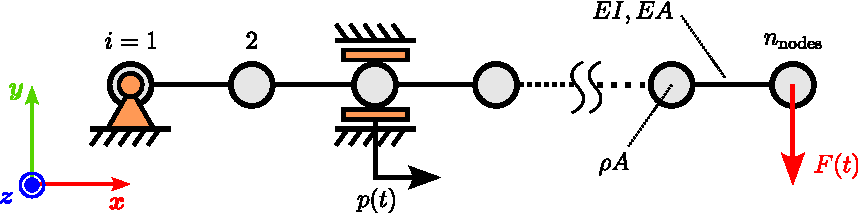
\includegraphics[scale=0.8]{PS_beam.pdf}
    \caption{Schematic representation of the mechanical problem under investigation. The nodes of the beam are drawn as circular disks. A beam, discretized using Euler-Bernoulli beam elements, is displacement-fixed on the left-hand side, while a joint slides along the beam, constraining its motion along the $y$-axis.}
    \label{fig:PS_beam}
\end{figure}

To obtain a global reduction basis, $n_\mathrm{snaps}$ so-called snapshots of the beam are sampled. For each snapshot, the sliding joint is placed at a different node of the beam, and the associated eigenvalue problem is solved. Ultimately, we obtain $\tPsi\,_i$, holding $n_\mathrm{eigvecs}$ eigenvectors of the system at the specific snapshot position.

Next, the snapshots $\tPsi\,_i$ are concatenated and we obtain the global reduction basis $\tPsi\in\mathbb{R}^{n_\mathrm{DOFs}\times n_\mathrm{global}}$ by performing a \ac{SVD}. Here, $n_\mathrm{global}$ is the number of global modes. The number of global modes can be varied, but
$n_\mathrm{global} \leq n_\mathrm{snaps} n_\mathrm{eigvecs}$
must hold.

After obtaining the global reduction basis, we set up the system:
\begin{align}
    \Mm \ddot\qv + \Km \qv + \Cm_\mathrm{q}\tp \tlambda = \fv \\
    \gv = \Null \eqdot
\end{align}
where $\qv$ denote the physical coordinates of the beam, $\Mm$ is the system mass matrix, and $\Km$ is the stiffness matrix. $\Cm_\mathrm{q}$ is the Jacobi-Matrix, being the derivatives of the binding vector $\gv$ with respect to the physical coordinates $\qv$. $\fv$ is the vector of external loads, being $\fv=\vtretp{\Null\tp}{F(t)}{0}\tp$ for our test case. After the global \ac{PMOR}, we obtain
\begin{align}
    \left(\Psi\tp\Mm\Psi\right) \ddot\qv + \left(\Psi\tp\Km\Psi\right) \qv + \left(\Cm_\mathrm{q}\Psi\right)\tp \tlambda = \Psi\tp\fv \\
    \gv = \Null \eqdot
\end{align}
Different formulations of the binding vector $\gv$ are tested and compared against the \ac{ANCF} sliding joint approach. Notably, the binding vector and thus the Jacobian are time-dependent. A naive formulation of the binding vector is that the $y$-coordinate of the node that is nearest to $p(t)$ is zeroed. This leads to jumping boundary conditions. The Hamiltonian of the beam, being the kinetic, strain, and potential energy of the system, is compared. Jumping boundary conditions highly increase the Hamiltonian. Thus, a binding vector with interpolation between the constraint nodes is proposed, which, together with the global reduction, shows good alignment with the \ac{ANCF} approach, see Figure~\ref{fig:R}. The results indicate that the global \ac{PMOR} is a viable option to model flexible \acp{MBS} with changing \acp{BC}. The next step is to fully integrate the presented approach within the \ac{FFRF}.

\begin{figure}[h]
    \centering
    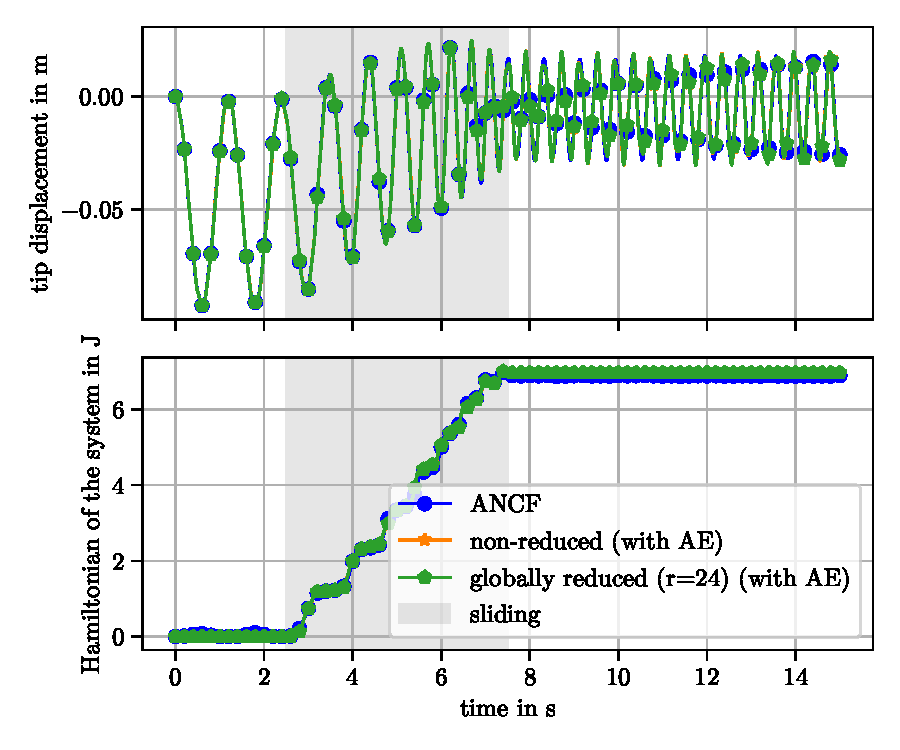
\includegraphics[scale=.8]{R.pdf}
    \caption{Preliminary test results of a globally reduced sliding beam. (Top) The displacement in the y-direction of the last node is shown. The \ac{ANCF} sliding joint approach is compared to a non-reduced beam and the globally reduced beam. Between the constraints, an interpolation is applied to avoid \textit{jumping} boundary conditions. (Bottom) The Hamiltonian of the system is shown. The gray area indicates the time slot in which the sliding joint moves.}
    \label{fig:R}
\end{figure}


% biliography
\begin{thebibliography}{aber}
\bibitem[1]{Orzechowski2017}
  Orzechowski, G.; Matikainen, M.; Mikkola, A.: 
  Inertia forces and shape integrals in the floating frame of reference formulation.
  \newblock Nonlinear Dyn., 2017.
  \newblock doi:\,10.1007/s11071-017-3355-y
\bibitem[2]{Steinbrecher2017}
  Steinbrecher, I.; Humer, A.; Vu-Quoc, L.: 
  On the numerical modeling of sliding beams: A comparison of different approaches.
  \newblock J. Sound Vib., 2017.
  \newblock doi:\,10.1016/j.jsv.2017.07.010.
\bibitem[3]{Gerstmayr2024}
  Gerstmayr, J.: 
  Exudyn – A C++ based Python package for flexible multibody systems.
  \newblock Multibody Syst. Dyn., 2024.
  \newblock doi:\,10.1007/s11044-023-09937-1
\end{thebibliography}
\end{document}
